\chapter{Descrição Geral do Sistema}

Este capítulo tem como objetivo descrever de forma geral o sistema, o escopo e as principais funções. A descrição geral do sistema deve abrange os itens a seguir. Como referência pode-se consultar e utilizar o modelo do RUP.



\section{Descrição do Problema}

Neste item deve ser descrito o problema que será resolvido com o desenvolvimento do sistema. As questões a seguir devem ser respondidas.

\begin{itemize}
	\item Quem é afetado pelo sistema?
	\item Qual é o impacto do sistema?
	\item Qual seria uma boa solução para o problema?
\end{itemize}
	


\section{Principais Envolvidos e suas Características}



\subsection{Usuários do Sistema}

Neste item deve ser descrito para qual tipo de empresa se destina o sistema, os tipos de usuários que utilizarão o sistema.
Estas informações são importantes para a definição de usabilidade G do sistema.

\subsection{Desenvolvedores do Sistema}
Neste item deve ser descrito os tipos de pessoas envolvidas em todo o desenvolvimento do sistema direta ou indiretamente.
Estas informações são importantes para a distribuição de responsabilidades e pontos-focais de desenvolvimento.


\section{Requisitos do Sistema}



\section{Fluxograma do Sistema Desenvolvido}



\section{Diagrama de Caso de Uso do Sistema }

{\color{red}Modelo de caso de Uso }

\begin{figure}[htb]
	\caption{\label{caso_uso}Caso de Uso do }
	\begin{center}
		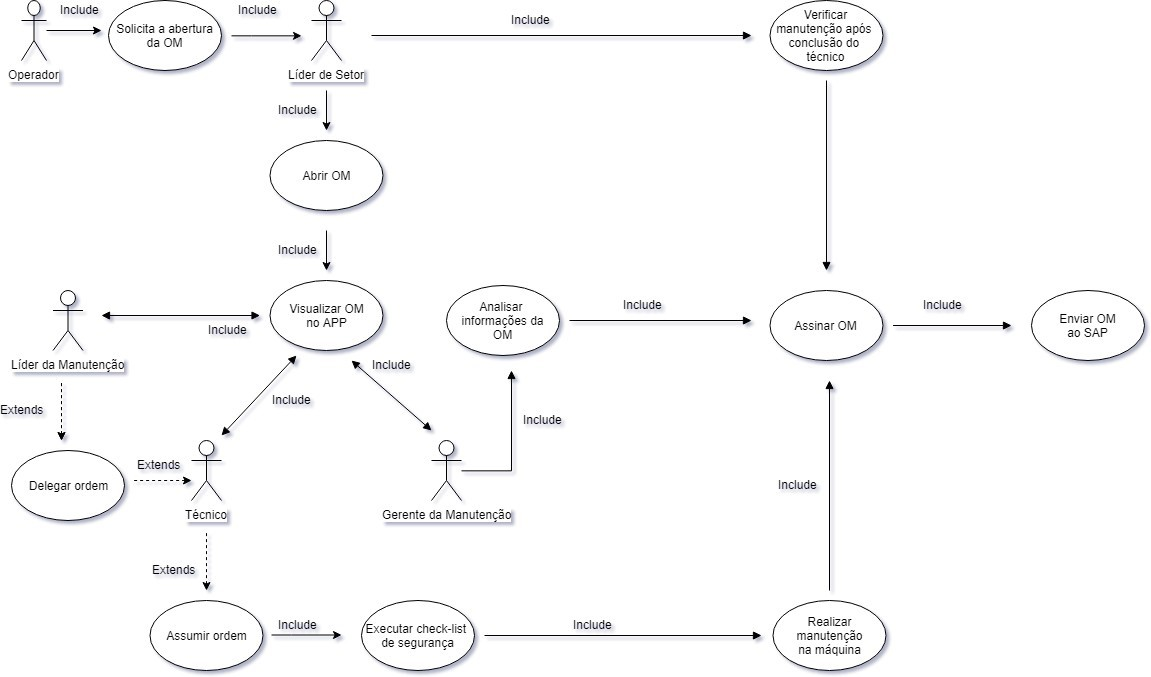
\includegraphics[scale=0.50]{./Figuras/caso-uso.png}
	\end{center}
	\legend{Fonte: Próprio Autor, 2019}
\end{figure}


\section{Diagrama de Classe}

\section{Métricas e  Cronograma do Projeto}

Neste item devem ser estimados os esforços necessários em termos de recursos alocados G e tempo para a obtenção do sistema. Para realizar a estimativa, indicam-se o uso de alguma técnica de métrica, como Pontos de Função ou Pontos de Caso de Uso.
Após os cálculos de métricas deve-se elaborar o cronograma detalhado do sistema, que contempla todas as tarefas descritas e os recursos alocados para cada tarefa, com datas para início e término de cada atividade. A seqüência das tarefas e a divisão entre os recursos devem ser realizadas de acordo com o processo de desenvolvimento de software escolhido para o desenvolvimento do sistema